
 	\subsection{ نتایج عددی} 
\begin{example}
	دستگاه  $2 \times 2 $ زیر را در نظر بگیرید. \\
	\begin{flalign}
	x_1 - x_2  & = (r, 2-r) \nonumber\\
	x_1 + 3x_2 & = (4 + r, 7 - 2r)\nonumber
	\end{flalign}
\end{example}
با توجه به روابط \ref{eq:4} می توان ماتریس S را به صورت زیر ساخت.\\
\begin{center}
	$
	S = 
	\begin{pmatrix}
	1 & 0 & 0 & 1 \\
	1 & 3 & 0 & 0 \\
	0 & 1 & 1 & 0 \\
	0 & 0 & 1 & 3 
	\end{pmatrix}
	$
\end{center}
با توجه به رابطه \ref{eq:8} می توان جواب دستگاه را به صورت زیر به دست آورد \\
$
X = 
\begin{pmatrix} 
\underline{x}_1\\
\underline{x}_2\\
\vdots\\
\underline{x}_n\\
-\overline{x}_1\\
\vdots\\
-\overline{x}_n	
\end{pmatrix} 
= S^{-1}{y} = 
\begin{pmatrix}
1.125 & -0.125 & 0.375 & -0.375 \\
-0.375 & 0.375 & -0.125 & 0.125 \\
0.375 & -0.375 & 1.125 & -0.125 \\
-0.125 & 0.125 & -0.375 & 0.375
\end{pmatrix}
\begin{pmatrix}
r \\
4 + r \\
r - 2\\
2r - 7
\end{pmatrix}
$
\begin{align}
\underline{x}_1 = 1.375 + 0.625r, \quad \overline{x}_1 = 2.875 - 0.875r\nonumber\\
\underline{x}_2 = 0.875 + 0.125r, \quad \overline{x}_2 = 1.375 - 0.375r\nonumber
\end{align}
می توان دید که دستگاه جواب فازی قوی دارد. \\ 
از آنجایی که ماتریس $ S $ غالب قطری اکید می باشد، طبق قضیه \ref{thm:3} هر دو روش ژاکوبی و گاوس سایدل همگرا هستند. برای محاسبات عددی نیاز به حاسبات سمبلک \LTRfootnote{symbolic} داریم. در اینجا ما از sympy \cite{sympy} استفاده کرده ایم. برای دیدن جزئیات پیاده سازی به پیوست مراجعه کنید. برای روش ژاکوبی داریم \\

	\begin{center}
	$ 
	M_{J} = 
	\begin{pmatrix}
	0 & 0 & 0 & 1 \\ 
	- \frac{1}{3} & 0 & 0 & 0 \\ 
	0 & 1 & 0 & 0 \\ 
	0 & 0 & -1/3 & 0 
	\end{pmatrix}
	\quad 
	C_{J} = 
	\begin{pmatrix}
	r \\ 
	\frac{r}{3} + \frac{4}{3} \\ 
	2 - r \\ 
	\frac{7}{3} - \frac{2r}{3}
	\end{pmatrix} \linebreak
	X^{k+1} = M_JX^{k} + C_{J} \linebreak 
	X_0 = \begin{pmatrix} 0 \\ 0 \\ 0 \\ 0 \end{pmatrix} \linebreak 
	X_1 = 
	\begin{pmatrix}
	r \\ 
	\frac{r}{3} + \frac{4}{3} \\ 
	2 - r \\ 
	\frac{7}{3} - \frac{2r}{3}
	\end{pmatrix} \linebreak
	X_2 = 
	\begin{pmatrix}
	\frac{r}{3} + \frac{7}{3} \\ 
	\frac{4}{3} \\ 
	\frac{10}{3} - \frac{2r}{3} \\ 
	\frac{5}{3} - \frac{r}{3}
	\end{pmatrix} \linebreak
	X_3 = 
	\begin{pmatrix}
	\frac{2r}{3} + \frac{5}{3} \\ 
	\frac{2r}{9} + \frac{5}{9} \\ 
	\frac{10}{3} - r \\ 
	\frac{11}{9} - \frac{4r}{9}
	\end{pmatrix} \linebreak
	X_4 = 
	\begin{pmatrix}
	\frac{5r}{9} + \frac{11}{9} \\ 
	\frac{r}{9} + \frac{7}{9}\\ 
	\frac{23}{9} - \frac{7r}{9} \\ 
	\frac{11}{9} - \frac{r}{3}
	\end{pmatrix} \linebreak
	X_5 = 	
	\begin{pmatrix}
	\frac{2r}{3} + \frac{11}{9} \\ 
	\frac{4r}{27} + \frac{25}{27}\\ 
	\frac{25}{9} - \frac{8r}{9} \\ 
	\frac{40}{27} - \frac{11}{27}
	\end{pmatrix} \linebreak
	$
	\end{center}
می توان دید ژاکوبی با ۵ تکرار به جواب همگرا شده. برای گاوس-سایدل به طور مشابه داریم 

	\begin{center}
		$ 
		M_{GJ} = 
		\begin{pmatrix}
		0 & 0 & 0 & 1 \\ 
		0 & 0 & 0 & -\frac{1}{3} \\ 
		0 & 1 & 0 & 0 \\ 
		0 & -\frac{1}{3} & 0 & 0 
		\end{pmatrix}
		\quad 
		C_{GJ} = 
		\begin{pmatrix}
		r \\ 
		\frac{4}{3} \\ 
		2 - r \\ 
		\frac{5}{3} - \frac{r}{3}
		\end{pmatrix} \linebreak
		X^{k+1} = M_JX^{k} + C_{J} \linebreak 
		X_0 = \begin{pmatrix} 0 \\ 0 \\ 0 \\ 0 \end{pmatrix} \linebreak 
		X_1 = 
		\begin{pmatrix}
		r \\ 
		\frac{4}{3} \\ 
		2 - r \\ 
		\frac{5}{3} - \frac{r}{3}
		\end{pmatrix} \linebreak
		X_2 = 
		\begin{pmatrix}
		\frac{2r}{3} + \frac{5}{3} \\ 
		\frac{r}{9} + \frac{7}{9}\\ 
		\frac{10}{3} - r \\ 
		\frac{11}{9} - \frac{r}{3}
		\end{pmatrix} \linebreak
		X_3 = 
		\begin{pmatrix}
		\frac{2r}{3} + \frac{11}{9} \\ 
		\frac{r}{9} + \frac{25}{27} \\ 
		\frac{25}{9} - \frac{8r}{9} \\ 
		\frac{38}{27} - \frac{10}{27}
		\end{pmatrix} \linebreak
		X_4 = 
		\begin{pmatrix}
		\frac{17r}{27} + \frac{38}{27} \\ 
		\frac{10r}{81} + \frac{70}{81}\\ 
		\frac{79}{27} - \frac{8r}{9} \\ 
		\frac{110}{81} - \frac{10r}{27}
		\end{pmatrix} \linebreak
		$
	\end{center}
	در شکل زیر جواب فازی دستگاه معادلات به همراه جواب های تقریبی به دست آمده از روش های ژاکوبی و گاوس-سایدل آمده. می توان دید که گاوس-سایدل تقریب بهتری با تعداد تکرار کمتر داشته. 
	
\begin{figure}[h] 
	\center 
	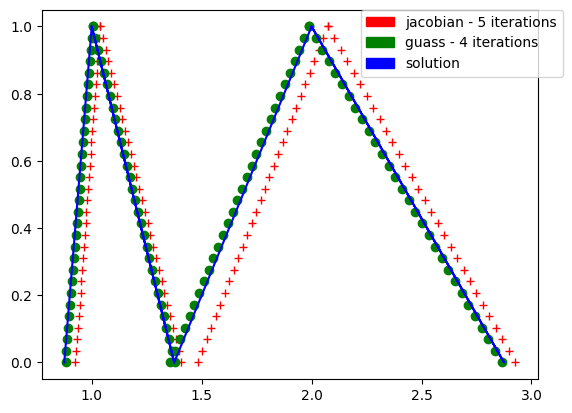
\includegraphics[width=0.7\linewidth]{assets/ex_1.png}
	\caption{مقایسه روش های تقریبی، معیار توقف $ \epsilon = 10^{-2} $}
\end{figure}

\begin{example}
	دستگاه  $3 \times 3 $ زیر را در نظر بگیرید. \\
	\begin{flalign}
	x_1 + x_2 - x_3  & = (r, 2-r) \nonumber\\
	x_1 - 2x_2 + x_3 & = (2 + r, 3)\nonumber\\
	2x_1 + x_2 + 3x_3 & = (-2, -1 - r)\nonumber
	\end{flalign}
\end{example}
با توجه به روابط \ref{eq:4} می توان ماتریس S را به صورت زیر ساخت.\\
\begin{center}
	$
	S = 
	\begin{pmatrix}
	1 & 1 & 0 & 0 & 0 & 1\\
	1 & 0 & 1 & 0 & 2 & 0\\
	2 & 1 & 3 & 0 & 0 & 0\\
	0 & 0 & 1 & 1 & 1 & 0\\
	0 & 2 & 0 & 1 & 0 & 1\\
	0 & 0 & 0 & 2 & 1 & 3
	\end{pmatrix}
	$
\end{center}
مشابه قبل داریم \\
\begin{align}
x_1 & = ( -2.31 + 3.62r,  4.69 - 3.38r),\nonumber\\
x_2 & = ( -0.62 - 0.77r, -1.62 + 0.23r),\nonumber\\
x_3 & = (  1.08 - 2.15r, -2.92 + 1.85r).\nonumber
\end{align}




با توجه به شکل ۲ می توان دید که $ x_1 $ برخلاف $ x_2, x_3 $ یک عدد فازی است
	
	\begin{figure}[h]
		\centering 
		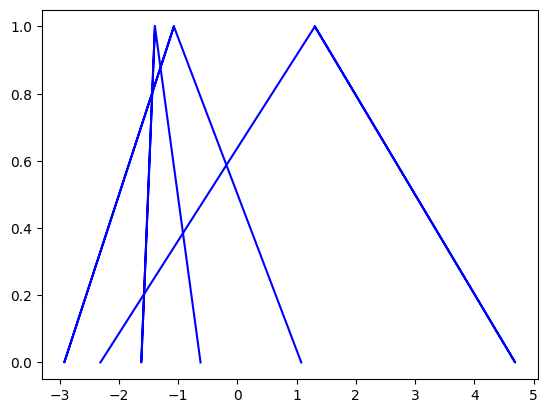
\includegraphics[width=0.6\linewidth]{assets/ex_2.png} 
		\caption{جواب فازی ضعیف دستگاه مثال ۳.۴.}
	\end{figure} 
		

	در نتیجه جواب دستگاه قبل به صورت زیر است. 
	\begin{align}
	u_1 & = ( -2.31 + 3.62r, 4.69 - 3.38r),\nonumber\\
	u_2 & = ( -1.62 + 0.23r  -0.62 - 0.77r),\nonumber\\
	u_3 & = ( -2.92 + 1.85r, 1.08 - 2.15r).\nonumber
	\end{align}	
	از آنجایی که ماتریس $ S $ غالب قطری اکید نمی باشد، تصمینی برای همگرایی روش های تکرار وجود ندارد. بعلاوه وارون ماتریس $ \left(L_B + D_B\right) $ وجود ندارد. در نتیجه نمی توانیم برای این مثال از روش های تکراری استفاده کنیم. 
	\begin{example}
		دستگاه  $3 \times 3 $ زیر را در نظر بگیرید. \\
		\begin{flalign}
		4x_1 + x_2 - x_3  & = (r, 2-r) \nonumber\\
		-x_1 + 3x_2 + x_3 & = (2 + r, 3)\nonumber\\
		2x_1 + x_2 + 3x_3 & = (-2, -1 - r)\nonumber
		\end{flalign}
	\end{example}
	\begin{center}
		$
		S = 
		\begin{pmatrix}
		4 & 1 & 0 & 0 & 0 & -1\\
		0 & 3 & 1 & -1 & 0 & 0\\
		2 & 1 & 3 & 0 & 0 & 0\\
		0 & 0 & -1 & 4 & 1 & 0\\
		-1 & 0 & 0 & 0 & 3 & 1\\
		0 & 0 & 0 & 2 & 1 & 3
		\end{pmatrix}
		$
	\end{center}
	مشابه قبل داریم \\
	\begin{align}
	x_1 & = (  0.1399r - 0.4125, -0.3217r + 0.0351),\nonumber\\
	x_2 & = (  0.2894r + 0.9125,  0.0970r + 1.1076),\nonumber\\
	x_3 & = ( -0.1897r - 0.6969, -0.1513r - 0.7353).\nonumber
	\end{align}
	
	از آنجایی که ماتریس $ S $ غالب قطری اکید است و همگرایی تضمین می شود می توان از روش های تکراری بار تقریب پاسخ استفاده کرد. شکل زیر دقت و سرعت همگرایی روش های تقریبی را برای این دستگاه معادلات نشان می دهد. می توانید با مراجعه به پیوست مقدار دقیق $ X $ در هر تکرار را تولید کنید. 
	
		
	\begin{figure}[h]
		\centering 
		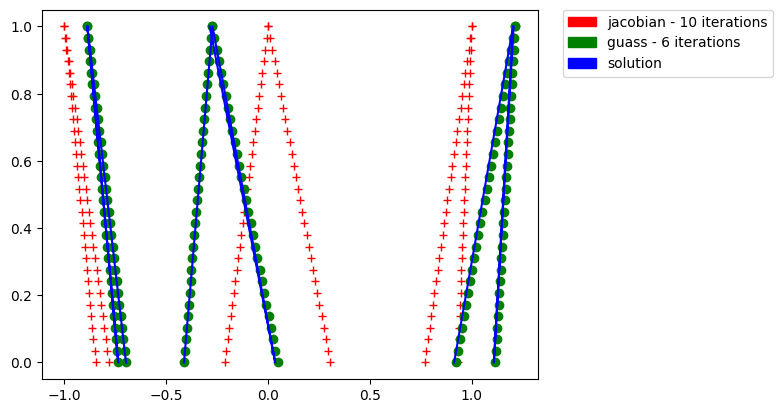
\includegraphics[width=0.9\linewidth]{assets/ex_3.png} 
		\caption{مقایسه روش های تقریبی، ‌در اینجا $ \epsilon=10^{-3} $ در نظر گرفته شده. همانطور که مشاهده می شود،‌ گاوس-سایدل با ۴ تکرار توانسته است جواب دقیق دستگاه را به خوبی تقریب بزند.}
	\end{figure} 
	
		
		\pagebreak
		